% Drawing 154/08-16 -- folder 154, batch 08, archive page 159 (PDF page 160).
% Transcription: dessin en couleur : deux facettes contiguës $F$ et $F'$, séparées et bordées par trois bandes verticales vert clair ; chacune est un cylindre dont les bords haut et bas sont des fuseaux rouges, traversé de courbes rouges verticales qui se croisent en huit ; des marques bleues aux coins de $F$ ; une droite horizontale (brune dans $F$, vert foncé dans $F'$) prolongée en pointillés bruns à gauche et à droite, marquée $D_i$ à droite, le point $a$ sur la bande commune ; des contours en tirets noirs, et les lettres $\delta$, $s$ dans $F$, $\delta'$, $s'$, $t'$ dans $F'$ ; les fuseaux de $F'$ se prolongent à droite en pointillés rouges
% Kind: two contiguous facets F and F', each a cylinder with red spindles at top and bottom and figure-eight curves. Method 2 (schematic redraw from the facsimile). Status: partial.
% Notes: A colour drawing: two contiguous facets F and F', separated and bordered by three vertical light green bands; each is a cylinder whose top and bottom edges are red spindles, crossed by vertical red curves that cross in figures of eight; blue marks at the corners of F; a horizontal line (dark grey, dotted beyond the facets, an arrow at the right end labelled D). The large pencil cross over the page is a cancellation stroke, not part of the drawing. Read from the page view; the figure-eight curves are schematic. Still differs from the facsimile: Read from the page view; the figure-eight curves are schematic.
% Coordinates: 1 unit = 1 mm = 1/100 of the crop width (bbox in page fractions: [0.134, 0.284, 0.42, 0.384]).
% Redrawn by Claude (claude-opus-5-5), issue #73, 2026-11-07; not checked by a human; not compiled (no TeX in the session).
% Revised by Claude (claude-opus-5-5) 2026-11-09 (issue #128) after Michel's check: vertices snapped to exact intersections (drawn points on their lines, meeting ends on the stroke they meet, near-concurrent lines through one computed point, curve ends on their rim); labels at \small as in folder 80 batch 3. Status: partial.
% Rights: reproduces part of the work -- behind RENDER_TRANSCRIPTS, never published by itself.
\documentclass[tikz,border=3pt]{standalone}
\usepackage{amsmath,amssymb}
\usetikzlibrary{patterns,arrows.meta}
\tikzset{Or/.style={orange!90!black}, Ye/.style={yellow!80!orange}, Lg/.style={green!60!black!70}, Dg/.style={green!45!black}, Br/.style={brown!80!black}, Rd/.style={red!85!black}, Bl/.style={blue!70!black}, Gy/.style={black!40}, pencil/.style={black!45}, struck/.style={black!35}, mark/.style={circle,draw,inner sep=1.3pt}, pt/.style={circle,fill,inner sep=0.9pt}, opt/.style={circle,draw,fill=white,inner sep=1.1pt}}
\begin{document}
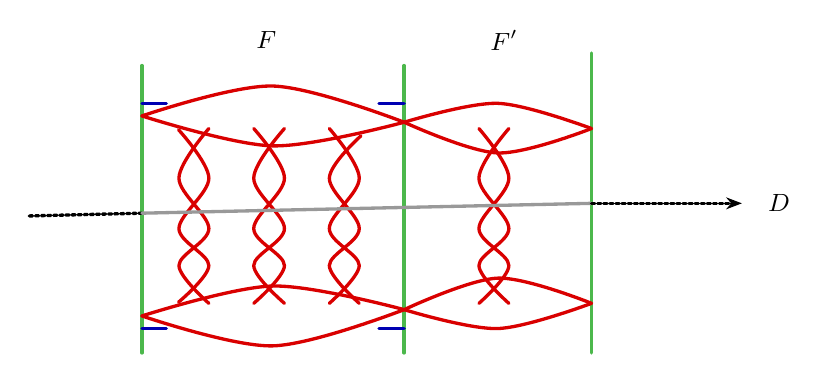
\begin{tikzpicture}[x=1mm,y=1mm,line cap=round,line join=round,font=\scriptsize]
\draw[Lg,very thick] (17.5,-9.5) -- (17.5,-46);
\draw[Lg,very thick] (50.8,-9.5) -- (50.8,-46);
\draw[Lg,very thick] (74.6,-7.9) -- (74.6,-46);
\draw[Rd,very thick] plot[smooth, tension=0.55] coordinates {(17.5,-15.9) (34.1,-12.1) (50.8,-16.7)};
\draw[Rd,very thick] plot[smooth, tension=0.55] coordinates {(17.5,-15.9) (34.1,-19.7) (50.8,-16.7)};
\draw[Rd,very thick] plot[smooth, tension=0.55] coordinates {(17.5,-41.3) (34.1,-37.5) (50.8,-40.5)};
\draw[Rd,very thick] plot[smooth, tension=0.55] coordinates {(17.5,-41.3) (34.1,-45.1) (50.8,-40.5)};
\draw[Rd,very thick] plot[smooth, tension=0.55] coordinates {(50.8,-16.7) (62.7,-14.3) (74.6,-17.5)};
\draw[Rd,very thick] plot[smooth, tension=0.55] coordinates {(50.8,-16.7) (62.7,-20.6) (74.6,-17.5)};
\draw[Rd,very thick] plot[smooth, tension=0.55] coordinates {(50.8,-40.5) (62.7,-36.5) (74.6,-39.7)};
\draw[Rd,very thick] plot[smooth, tension=0.55] coordinates {(50.8,-40.5) (62.7,-42.9) (74.6,-39.7)};
\draw[Rd,very thick] plot[smooth, tension=0.55] coordinates {(22.15,-17.65) (26,-23.8) (22.2,-30.2) (26,-34.9) (22.15,-39.55)};
\draw[Rd,very thick] plot[smooth, tension=0.55] coordinates {(26,-17.5) (22.2,-23.8) (26,-30.2) (22.2,-34.9) (26,-39.7)};
\draw[Rd,very thick] plot[smooth, tension=0.55] coordinates {(31.7,-17.5) (35.6,-23.8) (31.7,-30.2) (35.6,-34.9) (31.7,-39.7)};
\draw[Rd,very thick] plot[smooth, tension=0.55] coordinates {(35.6,-17.5) (31.7,-23.8) (35.6,-30.2) (31.7,-34.9) (35.6,-39.7)};
\draw[Rd,very thick] plot[smooth, tension=0.55] coordinates {(41.3,-17.5) (45.1,-23.8) (41.3,-30.2) (45.1,-34.9) (41.3,-39.7)};
\draw[Rd,very thick] plot[smooth, tension=0.55] coordinates {(45.32,-18.42) (41.3,-23.8) (45.1,-30.2) (41.3,-34.9) (45.1,-39.7)};
\draw[Rd,very thick] plot[smooth, tension=0.55] coordinates {(60.3,-17.5) (64.1,-23.8) (60.3,-30.2) (64.1,-34.9) (60.3,-39.7)};
\draw[Rd,very thick] plot[smooth, tension=0.55] coordinates {(64.1,-17.5) (60.3,-23.8) (64.1,-30.2) (60.3,-34.9) (64.1,-39.7)};
\draw[densely dotted,very thick] (3.2,-28.6) -- (17.5,-28.25);
\draw[Gy,very thick] (17.5,-28.25) -- (74.6,-27);
\draw[densely dotted,very thick,-{Stealth[length=2mm]}] (74.6,-27) -- (93.7,-27);
\node[inner sep=1pt] at (98.4,-27) {\small $D$};
\node[inner sep=1pt] at (33.3,-6.3) {\small $F$};
\node[inner sep=1pt] at (63.5,-6.3) {\small $F'$};
\draw[Bl,very thick] (17.5,-14.3) -- (20.6,-14.3);
\draw[Bl,very thick] (47.6,-14.3) -- (50.8,-14.3);
\draw[Bl,very thick] (17.5,-42.9) -- (20.6,-42.9);
\draw[Bl,very thick] (47.6,-42.9) -- (50.8,-42.9);
\end{tikzpicture}
\end{document}
